\documentclass[11pt]{article}
\usepackage[T1]{fontenc}
\usepackage{lmodern}
\usepackage{royden-report}
\usepackage{array}
\title{Dysthe CPU Pilot and A100 Research Decision}
\author{Water-wave numerical and learning experiments}
\date{26 October 2026}
\begin{document}
\maketitle
\noindent\textbf{Measured decision.} Short sequential spectral PINN solves are the strongest tested neural candidate for a prescribed inlet. They meet the pilot's sampled accuracy gates through $\xi=2$ on three independent test inlets, each with two optimization seeds. The numerical solver remains substantially faster and more accurate. FNO and PINO fail their held-out accuracy gates. The A100 continuation therefore prioritizes the slab PINN and preserves the operator results as controls.

\section{Question and model}
The goal is to investigate how long solutions remain numerically resolved, and whether neural approximations reproduce their phase, derivatives and sensitivity at useful cost. These calculations address finite distances and specified periodic fields. They do not prove global existence, uniqueness or nonlinear stability, or establish validity beyond Dysthe's asymptotic regime.

The fixed model, \texttt{water-wave-dysthe-spatial-v1}, is
\begin{equation}\label{eq:model}
\begin{split}
u_\xi={}&-i u_{\tau\tau}-i|u|^2u\\
 &-\epsilon\bigl(8|u|^2u_\tau+2u^2\overline{u_\tau}
                  +2iu|D_\tau|(|u|^2)\bigr).
\end{split}
\end{equation}
Here $u$ is the scaled free-surface envelope, $\tau\in[-20,20)$ is periodic retarded time, and $\xi$ is propagation distance. The Fourier multipliers are $ik$ for $\partial_\tau$ and $|k|$ for $|D_\tau|$, with $k=2\pi m/40$. The zero mode of the latter is zero. This is Fedele--Dutykh's free-surface spatial convention \cite{fedele}. Setting $\epsilon=0$ supplies the mathematical NLS control; the physical coordinate transformation is not invertible at zero steepness.

\begin{center}\small
\begin{tabular}{p{.24\textwidth}p{.66\textwidth}}\toprule
Test & Concrete purpose\\\midrule
Reference refinement & Separate neural error from numerical resolution error.\\
FNO versus PINO & Test whether a full PDE residual improves unseen-inlet prediction with the same backbone and training data.\\
NLS warm start & Test whether spending one quarter of a fixed budget on NLS improves a Dysthe PINN.\\
Global versus slabs & Test whether shorter intervals improve a per-inlet solve with the same total number of Adam updates.\\
Long propagation & Track numerical Sobolev norms and spectral resolution independently of neural models.\\
Signed perturbations & Measure sensitivity after checking perturbation size and numerical resolution.\\\bottomrule
\end{tabular}
\end{center}

\newpage
\section{Data, reference and neural implementations}
Eighteen deterministic initial fields comprise six bandlimited periodized chirped Gaussian packets, six carriers with asymmetric complex sidebands, and six smooth random complex Fourier fields. Four fields per family train the operators; one validates; one tests. All windows and refinements of an inlet remain in its split. There are \emph{three independent test fields}; two optimization seeds do not double that sample size.

Amplitude parameters lie in $[0.4,0.7]$, $\epsilon$ in $[0.02,0.05]$, packet widths in $[2.5,4]$, and chirps in $[-0.15,0.15]$. Initial fields are projected to $|m|\leq12$. Random fields have independent complex coefficients on $-6\leq m\leq6$. There is no fitted normalization, noise or external experimental data. This is a periodic experiment; no independence from the period or isolated whole-line packet behavior is asserted.

The reference uses Fourier differentiation, strict band $|m|<N/4$, and integrating-factor RK4 with linear multiplier $\exp(ik^2\Delta\xi)$. All fields were propagated through $\xi=4$ with $N=512$, $h=0.0025$, and saved every $0.05$. Independent comparisons at $(512,0.005)$ and $(256,0.0025)$ gave maximum discrepancies $2.44\times10^{-7}$ in relative $L^2$ and $2.19\times10^{-6}$ in relative $H^1$. Gates were $10^{-5}$ and $10^{-4}$. These are refinement comparisons, not rigorous continuum error bounds.

The learning grid has 128 points and explicit output band $|m|\leq24$. The full nonlinear residual uses 256 quadrature points on each periodic slice. Since the cubic RHS has bandwidth at most $3K$, $Q>6K$ resolves its squared norm for this trigonometric output. Generated RHS modes are not projected back to the learned band. PINN audits also use 512 points and 129 propagation slices. This addresses aliasing, not certification.

\paragraph{Operator comparison.}
The continuous-distance map is
\[
G_\theta(u_0,\epsilon,s)=S_sP_Ku_0+sP_KC_\theta(P_Ku_0,\epsilon,s).
\]
It enforces the projected inlet at $s=0$. The FNO has width 16, two Fourier/local layers, eight nonnegative latent Fourier modes, GELU activations and independent real/imaginary outputs \cite{fno}. Both conditions use the same architecture, seeds and 400 Adam updates. Windows begin in $[0,0.4]$, with offsets $0.05$ or $0.1$. Autonomous rollout repeats $0.1$ steps without reference resets.

The data loss is relative squared complex $L^2$ error plus $0.1$ times relative squared $H^1$ error. PINO adds $0.1$ times the full residual loss \cite{pino}, normalized by the detached predicted RHS mean square, floored at $10^{-8}$. Distance derivatives use a full-output Jacobian--vector product. Checkpoints minimize worst validation-field $H^1$ after rollout to $0.5$; mean seed scores rank operators.

\paragraph{Per-inlet comparison.}
A width-32, two-layer tanh network maps distance to complex Fourier coefficients correcting exact linear evolution. Each inlet receives a separate fit. Global and NLS-warm conditions fit $[0,2]$; the warm condition spends 100 of 400 updates at $\epsilon=0$. Four slabs of length $0.5$ receive 100 updates each and inherit the preceding predicted endpoint. Each update uses sixteen random distance slices. The loss uses the fixed inlet RHS mean square as scale. Checkpoints use only full-Dysthe residual validation, never numerical solution labels. Slabs respect forward propagation; they do not reproduce the specific causal weighting rule of \cite{causal}.

\newpage
\section{Measured PINN accuracy}
With normalized Fourier coefficients $\widehat v_m$, define
\[
\|v\|_{H^r}^2=40\sum_m(1+k_m^2)^r|\widehat v_m|^2,
\qquad E_r=\frac{\|u_{\rm pred}-u_{\rm ref}\|_{H^r}}{\|u_{\rm ref}\|_{H^r}}.
\]
The $L^2$ error is $E_0$. Phase and translation are not aligned away. Peak error is the relative difference of $\max_\tau|u|$. Gates require $E_0\leq1\%$, $E_1\leq5\%$ and peak error $\leq5\%$ on every held-out inlet and both seeds at all audited stations.

Table~\ref{tab:pinn} reports maxima over 41 saved stations through $\xi=2$, including intermediate points absent from the original summary. A frozen-checkpoint audit reconstructed 36 PINN fits and four operators. The largest slab interface jump was $1.56\times10^{-7}$ in relative $L^2$, consistent with float32 projection effects.

\begin{table}[h]\centering\small
\begin{tabular}{lrrrr}\toprule
 & Validation & \multicolumn{3}{c}{Test maxima (percent)}\\
Method & max. $E_0$ (\%) & $E_0$ & $E_1$ & Peak\\\midrule
Global PINN & 2.465 & 1.995 & 3.041 & 0.936 \\
NLS continuation & 3.095 & 2.074 & 3.560 & 1.285 \\
Four-slab PINN & 0.979 & 0.963 & 1.881 & 1.089 \\
\bottomrule\end{tabular}
\caption{Separate optimization per inlet; three validation and three test fields, two seeds. These are not operator generalization results.}\label{tab:pinn}
\end{table}

Slabs win on validation endpoint $H^1$ under either averaging over fields or averaging the seed-wise worst field. The latter score is $2.004\%$, versus $3.639\%$ for scratch and $4.446\%$ for NLS continuation. The audit made the reducer explicit because the initial protocol specified validation endpoint $H^1$ without a reducer. Raw case scores are preserved; the winner is unchanged. Test data did not select it.

\begin{center}
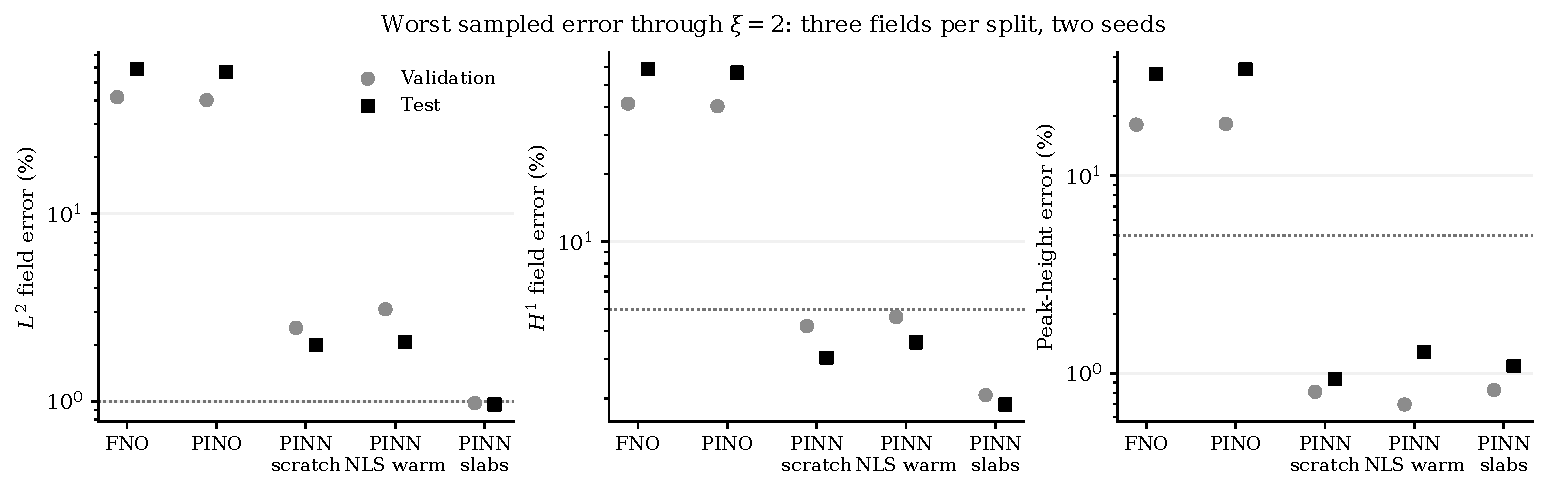
\includegraphics[width=.97\textwidth,height=.34\textheight,keepaspectratio]{figures/method-errors-xi2.pdf}
\end{center}

The supported conclusion is specific: shorter intervals improve this small spectral PINN under a fixed 400-update budget. NLS continuation does not improve the aggregate result under that budget. Neither establishes universal superiority. L-BFGS and self-scaled Broyden were not tested in this pilot. Each PINN approximates an interval on which its residual was optimized; this is not an unseen-distance forecast.

\newpage
\section{Operator failure and cost}
PINO's validation selection score is $9.588\%$, versus FNO's $10.002\%$: a small advantage that reverses for one seed. Every best operator checkpoint occurs at the first validation check, update 50. No test case/seed pair passes the gates through $\xi=0.5$. At $\xi=2$, worst field errors are $58.74\%$ for FNO and $56.62\%$ for PINO; at $\xi=4$ they exceed $100\%$.

\begin{center}
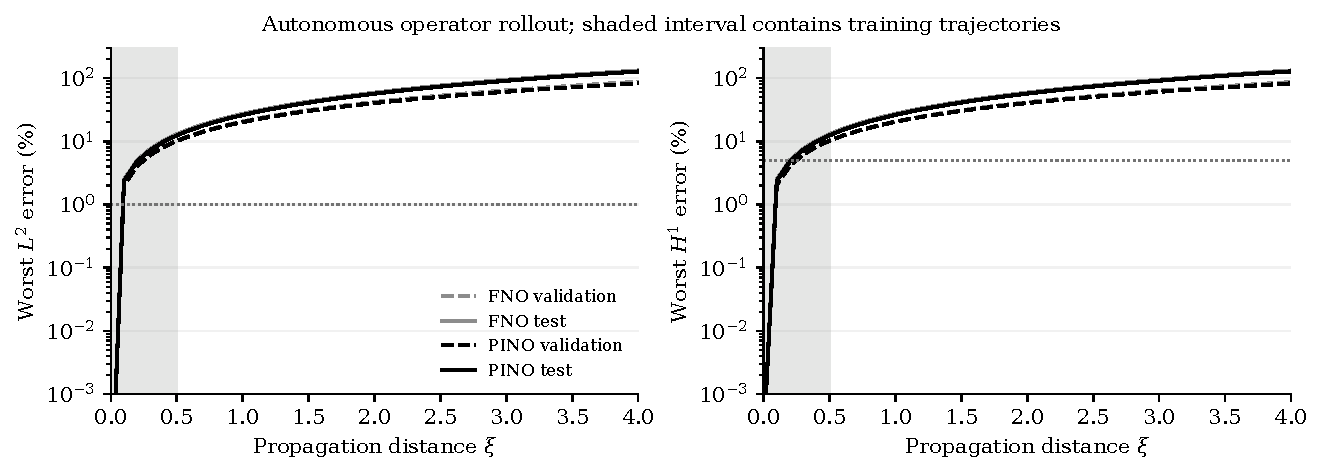
\includegraphics[width=.97\textwidth,height=.36\textheight,keepaspectratio]{figures/operator-growth.pdf}
\end{center}

This concerns twelve training inlets and a small optimization budget. It does not discredit operator learning in general. It does rule out presenting these trained operators as dependable long-distance predictors. A future study should add independent training fields, inspect phase/amplitude coverage, and test physical phase/translation augmentation with the same controls and a newly locked test sample. More epochs alone are unsupported by these validation curves.

\paragraph{Full cost matters.}
The slab PINN's recorded optimization time has median $1.258$ seconds per inlet. Warmed evaluation of 41 stations takes about $0.000645$ seconds. A complete coarse numerical solve on the same six fields to $\xi=2$ takes about $0.0294$ seconds, using five timing repetitions per field. Its worst test $H^1$ error is $4.62\times10^{-7}$. Per-inlet neural fitting is approximately 43 times slower even before full setup and checkpoint overhead. Cached evaluation is cheap; generating a new solution still requires fitting.

Training timers cover the update/validation loop and omit some setup, auditing and I/O. Initial operator and PINN training overlapped, each using two CPU threads. These are preliminary host wall-clock observations, not isolated hardware benchmarks. Subsequent inference/numerical timings were repeated after warmup. No optimized matched-accuracy solver speedup, A100 speedup, GPU memory measurement or throughput scaling is established. The numerical solver remains the practical baseline at this problem size.

\newpage
\section{Long-distance behavior and sensitivity}
Three validation fields were propagated numerically through $\xi=16$. Independent grid and step comparisons used $(N,h)=(1024,0.00125)$, $(512,0.00125)$ and $(1024,0.0025)$. Worst sampled relative $H^2$ discrepancies were $7.66\times10^{-13}$ for grid refinement and $4.87\times10^{-11}$ for step refinement.

\begin{center}
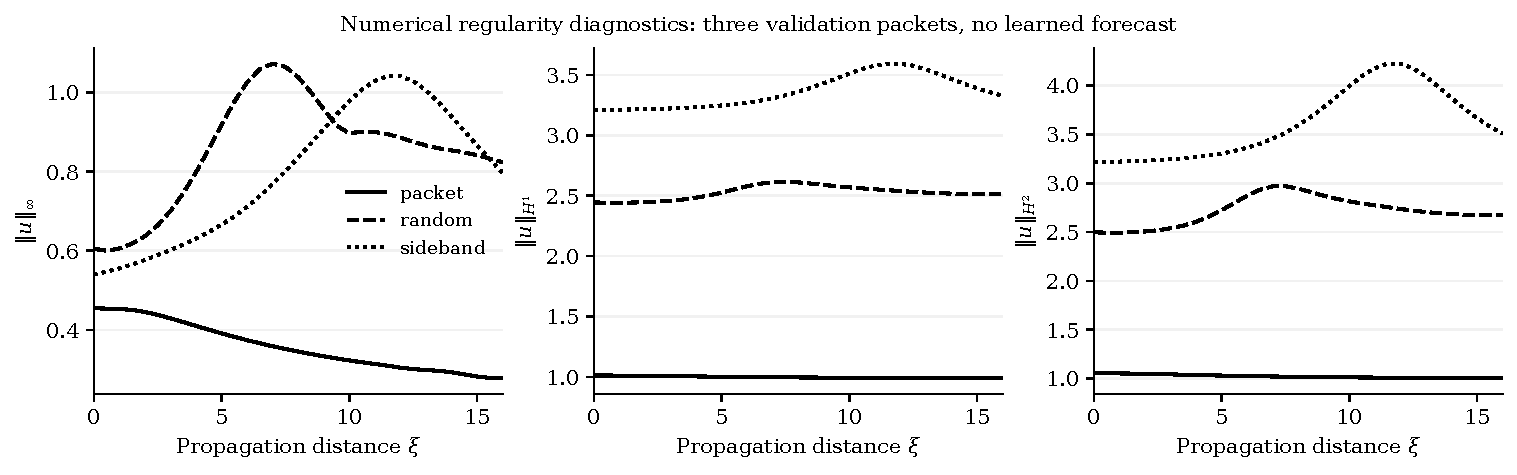
\includegraphics[width=.97\textwidth,height=.35\textheight,keepaspectratio]{figures/numerical-regularity.pdf}
\end{center}

The fields remain finite and resolved at sampled distances. Maximum sampled $H^2$ is about $4.224$, and effective steepness $\epsilon\|u\|_\infty$ is at most $0.0306$ in these runs. These diagnostics are not universal physical-validity thresholds. No learned prediction through $16$ was tested.

Each validation inlet was perturbed in a specified smooth complex direction $h$ with $\|h\|_{H^1}=1$. The signed centered response
\[
w_\delta(\xi)=\frac{S_\xi(u_0+\delta h)-S_\xi(u_0-\delta h)}{2\delta}
\]
was computed for $\delta=10^{-3}$ and $5\times10^{-4}$ through $\xi=4$. Maximum sampled $H^1$ amplification was $1.000$ for the packet, $2.025$ for the sideband field and $1.972$ for the random field. Signed-response grid/step discrepancies were below $7.78\times10^{-10}$; perturbation-halving discrepancy was below $3.82\times10^{-7}$. All met the declared 1\% response gate. This tests one direction per inlet over a finite distance.

\paragraph{Relation to existence.}
Every finite Fourier output is smooth in $\tau$ by construction. A PINN cannot detect a genuine loss of regularity merely by continuing to output a smooth field. Relevant empirical evidence comprises resolution-independent behavior, controlled spectral tails, full residuals, Sobolev norms and response convergence. Even these do not prove continuation for arbitrary distance. Proof requires an applicable well-posedness/continuation argument with controlled norms, or validated a-posteriori bounds including truncation and stability. No such certificate is claimed here.

\newpage
\section{A100 continuation and reproduction}
The next experiment is a proposed extension of the selected slab PINN. A new seed generates 36 fields: six validation and six test inlets are reserved, with three optimization seeds. It fits through $\xi=4$ in eight slabs, with 3200 Adam updates, width 64, depth three, 64 collocation slices, 256 profile samples and output band $K=48$. These simultaneous changes define a scaling/robustness challenge, not an ablation assigning improvement to one resource.

All 36 proposed reference trajectories were qualified on CPU through $\xi=8$ using $N=1024$, $h=0.00125$ and independent grid/step comparisons. Maximum $L^2$ discrepancy was about $4.3\times10^{-8}$. Neural training and CUDA restart behavior remain untested.

\begin{center}\small
\begin{tabular}{p{.25\textwidth}p{.65\textwidth}}\toprule
Next test & Goal and decision\\\midrule
CPU/GPU parity & Verify the complete RHS and usable distance/parameter derivatives before interpreting acceleration.\\
New-inlet slab solves & Require all sampled gates on six untouched test inlets and three seeds through $\xi=4$. Retain failures.\\
Bandwidth/slab audit & Recompute difficult cases with more modes and shorter slabs; compare actual reference errors and full residuals.\\
Cost and memory & Record reference generation, optimization, evaluation and peak GPU memory separately; compare full cost with the CPU solver.\\
Perturbation extension & Qualify numerical responses before comparing separately optimized PINNs, whose differences include fitting error.\\\bottomrule
\end{tabular}
\end{center}

The launcher requests one \texttt{gpu2} A100 of type \texttt{A100-PCI-40GB}, four CPU cores, 16 GB host memory and two hours. The latter choices are initial allocations, not measurements. For \texttt{gpu1}, override both partition and type to \texttt{A100-SXM4-40GB}. The GPU strings follow the official AI.Panther guide \cite{cluster}. No account is guessed and no job was submitted. The allocation first checks CUDA/CPU RHS agreement and actual PINN JVP/backpropagation.

Experiments pin published core and learning commits. Raw arrays and checkpoints remain outside Git. Included JSON/CSV files retain configurations, groups, refinement evidence, source hashes and checkpoint hashes, curves and errors. Resume restores Adam, weights and random states; exact next-step CPU restart was tested. GPU equivalence still needs measurement.

From the reviewed experiments checkout and a prepared CUDA environment:
\begin{verbatim}
export DYSTHE_PYTHON=/absolute/path/to/venv/bin/python
export RUN_DIR=runs/a100-pilot-01
sbatch cluster/run-a100-pilot.sbatch
\end{verbatim}
Environment preparation, optional account and resume instructions are in \texttt{cluster/README.md}. This directory contains the editable report, style, table and vector PDF figures.

\newpage
\section*{Verification and provenance}
The 32 core checks, 11 learning checks and six focused campaign reproducibility checks passed. These include an independent nonconstant mean-flow calculation, exact plane-wave phase, Fourier interpolation, differentiable residuals, phase-sensitive error and checkpoint recovery. The 76 saved best checkpoints were reconstructed for the accuracy audit. A separate completed-run replay preserved all 96 slab best/last checkpoint hashes and reproduced its metrics; a unit test separately verified the identical next optimizer update after CPU restart. The completed-run replay does not test interruption on CUDA.

The report was compiled with pdfLaTeX, extracted for content checks and rendered for inspection of every page. All three included figures are vector PDFs with embedded fonts. The original training-driver hash and the later replay-driver hash are recorded separately; configuration guards and A100 controls were added after the CPU training. The original run metadata is retained. Raw arrays and checkpoint files are stored locally in the ignored run directory and can be regenerated by the documented commands.

The published core dependency is
\begin{center}\small\texttt{a47a42321475feb6bc55031f4b752419f4b7fda9}.\end{center}
The published learning dependency is
\begin{center}\small\texttt{db7274f8cfe959cf187351f56b3dd4bf89f0e9b4}.\end{center}
The experiments workstream is \texttt{codex/cpu-pilot-a100}. Its cluster launcher passed shell syntax and simulated scheduler-dispatch checks, including rejection guards. Those checks do not validate an actual Slurm allocation, driver, GPU execution, wall time or memory requirement. No cluster job was submitted.

\begin{thebibliography}{9}\small
\bibitem{fedele} F. Fedele and D. Dutykh (2011; revised 2012), \emph{Hamiltonian description and traveling waves of the spatial Dysthe equations}. \url{https://arxiv.org/abs/1110.3605}.
\bibitem{fno} Z. Li et al. (2020; revised 2021), \emph{Fourier Neural Operator for Parametric Partial Differential Equations}. \url{https://arxiv.org/abs/2010.08895}.
\bibitem{pino} Z. Li et al. (2021; revised 2023), \emph{Physics-Informed Neural Operator for Learning Partial Differential Equations}. \url{https://arxiv.org/abs/2111.03794}.
\bibitem{causal} S. Wang, S. Sankaran and P. Perdikaris (2022), \emph{Respecting causality is all you need for training physics-informed neural networks}. \url{https://arxiv.org/abs/2203.07404}.
\bibitem{cluster} Florida Institute of Technology, \emph{AI.Panther submission guide}, consulted 26 October 2026. \url{https://help.fit.edu/TDClient/39/Portal/KB/PrintArticle?ID=2107}.
\end{thebibliography}
\end{document}
